
\chapter{Simulator architecture}
\label{sec:simulator}

The implemented simulator consists of two main components:

\begin{itemize}
	\renewcommand{\labelitemi}{$\bullet$}
	
	\item \textbf{Simulator}
	\item \textbf{Simulator master}
	
\end{itemize}

The simulator component is a container running multiple node instances, providing an interface for performing operations on the simulator instance and on individual nodes. The operations include creating new nodes (joining the DHT), dropping nodes (simulating failures) and running operations in individual nodes' contexts (sending messages, performing lookup, search and the DHT operations, as well as calling nodes' extensions, background processes, running the recovery procedure and leaving the system). The simulator also maintains a number of counters: the total number of messages sent, the number of messages delivered/lost, and the route lengths (using an additional received message processor and message send processor (\emph{StatReceivedMessageProcessor}, \emph{StatMessageSendProcessor}), which collect information about messages being sent and received).

Multiple simulator instances may be connected to each other, and the nodes maintained by individual simulators may form a common DHT system, using virtual network addresses, determining on which simulator instance nodes are located, and identifying the nodes within individual simulators. The communication method (virtual network layer) between nodes located within the same simulator instance, as well as located in separate simulator instances, is defined by implementing a simulator-specific network proxy.

\begin{figure}
\centering
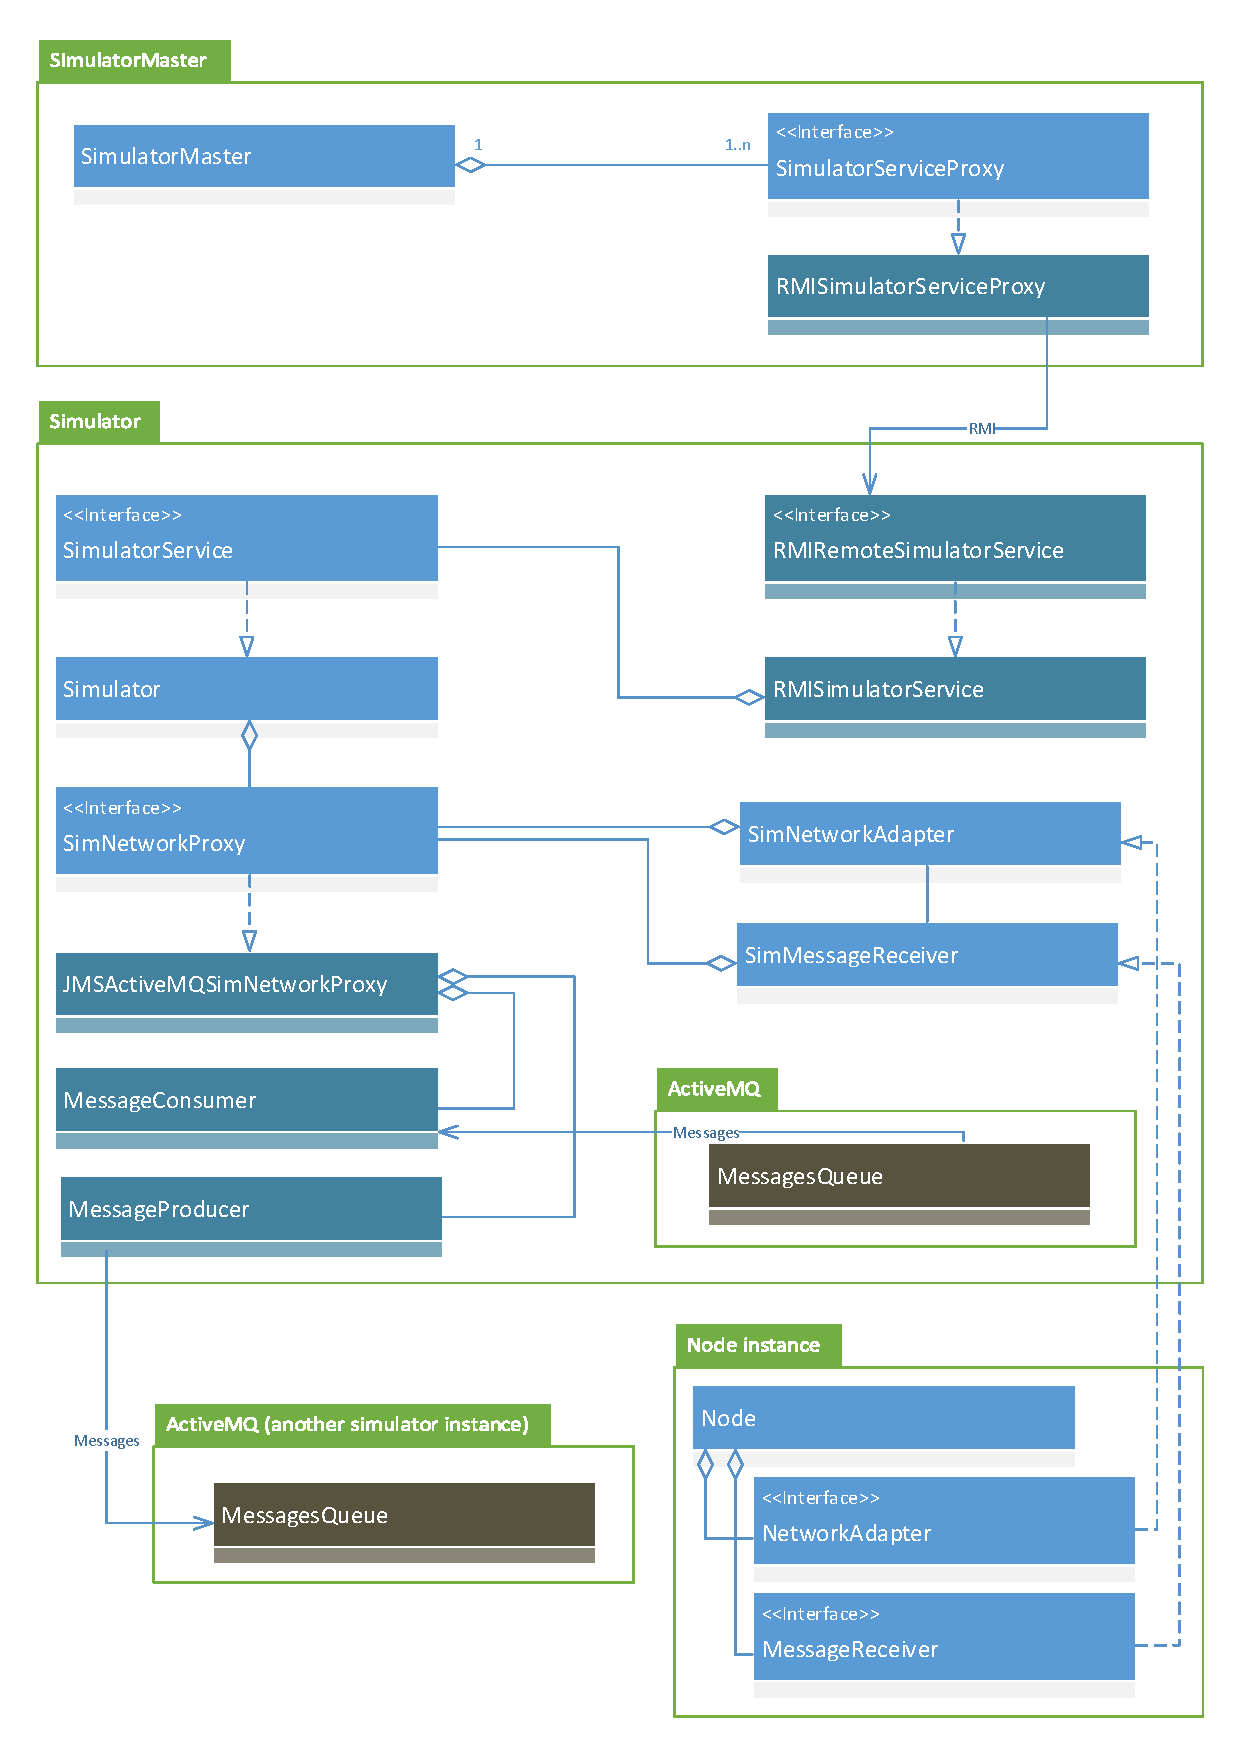
\includegraphics[trim = 5mm 0mm 5mm 5mm, clip, scale=.79]{img/HyCubeSimulator.pdf}
\caption{Simulator architecture}
\label{fig:simHyCubeSimulatorArchitecture}
\end{figure}

Figure \ref{fig:simHyCubeSimulatorArchitecture} presents the architecture of the simulator. The central object is the simulator master (an instance of the \emph{SimulatorMaster} class). The simulator master provides methods establishing connections to individual simulator instances and performing operations on them, using an internal simulator service proxy object (implementing the interface \emph{SimulatorServiceProxy}) and an appropriate service (stub) passing requests to the simulator object. The simulator instances are identified by the simulator ID and the connection information is determined by the connection string provided to the simulator master (the interpretation is \emph{SimulatorServiceProxy} implementation dependent). The simulator service proxy object is created by the simulator master through a factory object (\emph{SimulatorServiceProxyFactory}), passed to the \emph{initialize} method of \emph{SimulatorMaster}. The proxy object connects to the simulator (an instance of \emph{Simulator} class implementing the \emph{SimulatorService} interface) through a stub object (on the simulator side), which maintains a reference to the simulator instance and passes requests to the simulator object.

A message being sent is passed by node's network adapter to the simulator network proxy object, maintained by every simulator (implementing \emph{SimNetworkProxy} interface), which transfers the message to the appropriate simulator instance (the communication method is determined by the network proxy implementation). The message receiver of the receiving simulator also retrieves the message using the abstraction of the network proxy, and upon receiving the message, passes it to the network adapter of the appropriate node. The simulator network proxy instance is defined upon the simulator object initialization and is responsible for establishing connections between simulator instances, as well as for sending messages to nodes and receiving messages - the network proxy object is bound to simulator network adapter and simulator message receiver instances - \emph{SimNetworkAdapter} and \emph{SimMessageReceiver} - the network adapter and message receiver implementations that use the simulator network proxy object for sending and receiving messages. The simulator network proxy implementation defines the network layer (how simulated nodes communicate with each other), and the simulator logic is independent of this implementation. The node network address is defined by \emph{SimNetworkAdapter} and \emph{SimMessageReceiver} as a string in the following format: \emph{SIMULATOR\_ID:NODE\_SIM\_ID}, where \emph{SIMULATOR\_ID} is the simulator ID (4-character ISO-8859-1 string) and the \emph{NODE\_SIM\_ID} (16-character ISO-8859-1 string) is the simulation identifier of the node. The simulator ID is specified when the simulator object is created, and the simulation node ID is specified when the node is created (passed through the simulator service proxy to the simulator instance). Based on the simulator ID, the simulator network proxy of the sending node (simulator instance maintaining the sending node) should be able to determine to which simulator instance messages should be transferred, and, upon receiving a message, the \emph{SimMessageReceiver} instance (of the simulator maintaining the recipient) is responsible for determining the node (network adapter instance) to which the message should be passed. \emph{SimNetworkAdapter} and \emph{SimMessageReceiver} operate on network addresses represented by \emph{SimNodePointer} class (implementing \emph{NetworkNodePointer}), and the binary representation of the address is the concatenation of byte representations of simulator id and simulation node id, encoded in ISO-8859-1 (20 bytes long). Connections between individual simulators are established by calling the simulator master's methods, specifying simulator network proxy specific connection strings, defining the connections. The simulator master passes connection requests to individual simulators, which pass the requests to their simulator network proxy objects, responsible for establishing and maintaining connections (the simulator master uses the network proxy abstraction, the connection realization is network proxy implementation dependent).

The simulator service proxy implemented in the simulator is based on the Java RMI technology and is represented by class \emph{RMISimulatorServiceProxy} (implementing \emph{RMISimulatorSereviceProxy}). The factory object passed to the simulator master initializer is an instance of class \emph{RMISimulatorServiceProxyFactory}. The RMI proxy connects to the stub object of class \emph{RMISimulatorService}, implementing the remote interface \emph{RMIRemoteSimulatorService}. The \emph{RMISimulatorService} object internally maintains a reference to an object implementing the \emph{SimulatorService} interface (the simulator), passed to the class constructor upon creation. The stub object simply passes the calls received to the simulator object. The connection string format expected by \emph{RMISimulatorSereviceProxy} is the standard URL format defining RMI remote objects: \emph{//host:port/name}.

The simulator network proxy implementation provided with the library is based on the JMS queues (ActiveMQ implementation). The network proxy object maintained by the simulator object is an instance of class \emph{JMSActiveMQSimNetworkProxy} (implementing \emph{SimNetworkProxy}). Instances of the network proxies establish connections to the local ActiveMQ queues (consumer), and to the queues of all connected (including self) simulator instances (as a producer). Whenever a message is sent, the node proxy object sends it to the ActiveMQ queue (packed in the instance of the \emph{SimMessage} class) of the appropriate simulator, and message receiver instances, through the abstraction of the network proxy, receive the messages from the local ActiveMQ queues. The connection string format expected by \emph{JMSActiveMQSimNetworkProxy} is: \emph{protocol://host:port[queue]}, where \emph{protocol}, \emph{host} and \emph{port} define the JMS connection, and \emph{queue} is the message queue name, for example: \emph{tcp://testmachine01:51001[SimMessages]}.

The simulator application (service) - class \emph{SimulatorRemoteServiceApp1} creates an instance of \emph{JMSActiveMQSimWakeableNetworkProxy}, initializes a \emph{Simulator} instance and creates an instance of \emph{RMISimulatorService}, passing the reference to the simulator to it and exposing the remote object through RMI.

The master application (\emph{SimulatorMasterApp1} class) creates a simulator master (\emph{SimulatorMaster} class) instance and runs a simulation script - a class implementing the \emph{Simulation} interface specified as a command line argument (by calling its \emph{runSimulation} method, passing the simulator master object and the remaining command line parameters to it). The simulation script (implementation of the \emph{Simulation} interface) may connect to individual simulator instances and realize any possible simulation scenarios.






% ex: set tabstop=4 shiftwidth=4 softtabstop=4 noexpandtab fileformat=unix filetype=tex encoding=utf-8 fileencodings= fenc= spelllang=pl,en spell:

